\documentclass[11pt,letterpaper, leqno]{article}
\usepackage{latexsym}
\usepackage{amsmath}
\usepackage{amssymb}
\usepackage{amsthm}
\usepackage{listings}

\topmargin -0.25in
\textheight 8.5in
\oddsidemargin 0.0in
\textwidth 6.5in

\RequirePackage{amsthm,amsmath,amsfonts,amssymb}
%\RequirePackage[numbers]{natbib}
\RequirePackage[authoryear]{natbib}%% uncomment this for author-year citations
\RequirePackage{graphicx}%% uncomment this for including figures

\usepackage{tikz}
\usepackage{graphicx}
\usepackage{natbib}
\usepackage{authblk}
\usepackage[english]{babel}
\bibliographystyle{abbrvnat}
\setcitestyle{authoryear,open={(},close={)}}
\usepackage{hyperref}
\hypersetup{colorlinks,citecolor=blue,urlcolor=blue}

% For the algorithm table
\usepackage{algorithm,algcompatible,amsmath}
\DeclareMathOperator*{\argmax}{\arg\!\max}
\DeclareMathOperator*{\argmin}{\arg\!\min}
% https://tex.stackexchange.com/q/83169/5764
\algnewcommand\INPUT{\item[\textbf{Input:}]}%
\algnewcommand\OUTPUT{\item[\textbf{Output:}]}%
%

% the settings of tikz is used for the optimization of the graphs  
\usetikzlibrary{shapes, arrows, calc, arrows.meta, fit, positioning} % these are the parameters passed to the library to create the node graphs  
\tikzset{  
    -Latex,auto,node distance =1.5 cm and 1.3 cm, thick,% node distance is the distance between one node to other, where 1.5cm is the length of the edge between the nodes  
    state/.style ={ellipse, draw, minimum width = 0.9 cm}, % the minimum width is the width of the ellipse, which is the size of the shape of vertex in the node graph  
    point/.style = {circle, draw, inner sep=0.18cm, fill, node contents={}},  
    bidirected/.style={Latex-Latex,dashed}, % it is the edge having two directions  
    el/.style = {inner sep=2.5pt, align=right, sloped}  
}  


\newtheorem{theorem}{Theorem}
\newtheorem{acknowledgement}[theorem]{Acknowledgement}
%\newtheorem{algorithm}[theorem]{Algorithm}
\newtheorem{axiom}[theorem]{Axiom}
\newtheorem{problem}[theorem]{Problem}
\newtheorem{remark}{Remark}
\newtheorem{claim}[theorem]{Claim}
\newtheorem{conclusion}[theorem]{Conclusion}
\newtheorem{condition}[theorem]{Condition}
\newtheorem{conjecture}[theorem]{Conjecture}
\newtheorem{corollary}{Corollary}
\newtheorem{criterion}[theorem]{Criterion}
\newtheorem{definition}{Definition}
\newtheorem{example}{Example}
\newtheorem{exercise}[theorem]{Exercise}
\newtheorem{lemma}{Lemma}
\newtheorem{proposition}{Proposition}
\newtheorem{thm}{Theorem}[section]
\newtheorem{lem}{Lemma}[section]
\newtheorem{prop}{Proposition}[section]
\newtheorem{defn}{Definition}[section]
\newtheorem{ex}{Example}[section]
\newtheorem{cor}{Corollary}[section]
\newtheorem{rem}{Remark}[section]
\newtheorem{rems}{Remarks}[section]
\numberwithin{equation}{section} 
\numberwithin{theorem}{section}
\numberwithin{lemma}{section} 
\numberwithin{corollary}{section}
\numberwithin{definition}{section}
\numberwithin{proposition}{section} 
\numberwithin{remark}{section}
\numberwithin{example}{section}
\newtheorem{assumption}{Assumption}
\DeclareMathOperator\supp{supp}

%\newcommand{\ex}{{\bf\sf E}}            %% expectation
\newcommand{\bfp}{{\bf P}}
\newcommand{\bfr}{{\bf R}}
\newcommand{\Var}{{\rm Var}}            %% 
\newcommand{\Cov}{{\rm Cov}}            %% 
\newcommand{\calc}{{\cal C}}            %%
\newcommand{\cald}{{\cal D}} 
\newcommand{\calf}{{\cal F}}            %%
\newcommand{\call}{{\cal L}}            
\newcommand{\al}{\alpha}                %%
\newcommand{\bt}{\beta}                %%
\newcommand{\ga}{\gamma}                %% abbreviated
\newcommand{\dt}{\delta}                %% greek letters
\newcommand{\la}{\lambda}               %%
\newcommand{\ep}{\epsilon}              %%
\newcommand{\sig}{\sigma}               %%
\newcommand{\tri}{\triangle}
\newcommand{\om}{\omega}                %%
\newcommand{\ra}{\rightarrow}           %%
\newcommand{\lra}{\longrightarrow}
\newcommand{\Ra}{\Rightarrow}           %% arrows
\newcommand{\subs}{\subseteq}           %% subset or equal to
\newcommand{\eqdef}{\stackrel{\triangle}{=}}
\newcommand{\hY}{\hat{Y}}
\newcommand{\hp}{\hat{p}}
\newcommand{\hX}{\hat{X}}
\newcommand{\hy}{\hat{y}}
\newcommand{\hQ}{\hat{Q}}
\newcommand{\Zh}{\hat{Z}}
\newcommand{\hla}{\hat{\lambda}}
\newcommand{\starti}{\parindent0pt\it}  %% start an italic line
\newcommand{\startb}{\parindent0pt\bf}  %% start a boldface line
\newcommand{\tril}{\triangle^-}
\newcommand{\trir}{\triangle^+}
\newcommand{\trilr}{\triangle^{\pm}}
\newcommand{\realR}{{{\rm I}\;\!\!\!{\rm R}}}
\newcommand{\probP}{{{\rm I}\;\!\!\!{\rm P}}}
\newcommand{\filtF}{{{\rm I}\;\!\!\!{\rm F}}}
\newcommand{\expeE}{{{\rm I}\;\!\!\!{\rm E}}}
\newcommand{\noin}{{\noindent}}
\newcommand{\doty}{{\dot{y}}}
\newcommand{\doth}{{\dot{h}}}
\newcommand{\dotx}{{\dot{x}}}
\newcommand{\dotu}{{\dot{u}}}
\newcommand{\dotf}{{\dot{f}}}
\newcommand{\dotg}{{\dot{g}}}
\newcommand{\ddoty}{{\ddot{y}}}
\newcommand{\ddoth}{{\ddot{h}}}
\newcommand{\ddotx}{{\ddot{x}}}
\newcommand{\ddotf}{{\ddot{f}}}
%\newcommand{\Var}{{\mbox{Var}}}
%\newcommand{\Cov}{{\mbox{Cov}}}
\newcommand{\T}{\intercal}

\newcommand{\ans}[1]{\boxed{\text{#1}}}
\newcommand{\vecs}[1]{\langle #1\rangle}
\renewcommand{\hat}[1]{\widehat{#1}}
\newcommand{\F}[1]{\mathcal{F}(#1)}
\renewcommand{\P}{\mathbb{P}}
\newcommand{\R}{\mathbb{R}}
\newcommand{\E}{\mathbb{E}}
\newcommand{\Z}{\mathbb{Z}}
\newcommand{\ind}{\mathbbm{1}}
\renewcommand{\qed}{\quad \blacksquare}
\newcommand{\brak}[1]{\left\langle #1 \right\rangle}
\newcommand{\bra}[1]{\left\langle #1 \right\vert}
\newcommand{\ket}[1]{\left\vert #1 \right\rangle}
\newcommand{\abs}[1]{\left\vert #1 \right\vert}
\newcommand{\mfX}{\mathfrak{X}}
\newcommand{\V}{\mathbb{V}}
\usepackage{tcolorbox}
\tcbuselibrary{breakable, skins}
\tcbset{enhanced}
\newenvironment*{tbox}[2][gray]{
    \begin{tcolorbox}[
        parbox=false,
        colback=#1!5!white,
        colframe=#1!75!black,
        breakable,
        title={#2}
    ]}
    {\end{tcolorbox}}


\begin{document}
\begin{center}
{\bf \Large APMA1690: ~~Homework \# 10 ~~~(Due by 11pm December 8)}
\end{center}
\[\]
\medskip


\begin{center}
    ``\textit{Subtle is the Lord, but malicious he is not.}"
\end{center}
\begin{flushright}
--- Albert Einstein
\end{flushright}


\section{Review}

I would suggest you go through the review section before going to the problem set.

\subsection{Manifold Hypothesis}\label{section: Manifold Hypothesis}

Every science is based on one or several assumptions. Manifold learning (also known as `dimension reduction') is not an exception --- manifold\footnote{The precise definition of \href{https://en.wikipedia.org/wiki/Manifold}{manifolds} is quite technical and beyond the scope of APMA 1690. You may just roughly think of a manifold as a surface/curve/hyperplane/line.} learning is based on the so-called `manifold hypothesis:' \textit{high dimensional data tend to lie in the vicinity of a low dimensional manifold} \citep{fefferman2016testing}.\footnote{The first author \href{https://en.wikipedia.org/wiki/Charles_Fefferman}{Charles Fefferman} achieved a full professorship at the University of Chicago at the age of 22, making him the youngest full professor ever appointed in the United States. Fefferman entered the University of Maryland at age 14, graduated with degrees in mathematics and physics at 17, and earned his PhD in mathematics three years later from Princeton University.} The `high dimension' is usually referred to as the `extrinsic dimension,' and the `low dimension' is usually referred to as the `intrinsic dimension.' 

\subsection{Notations}

\begin{itemize}
    \item $d$ and $D$ are two positive integers satisfying $d<D$. Hereafter, $d$ denotes an intrinsic dimension, and $D$ denotes an extrinsic dimension.

\item For any matrix $\boldsymbol{A}$, its \href{https://en.wikipedia.org/wiki/Transpose}{transpose} is denoted as $\boldsymbol{A}^\T$.

    \item For any $\boldsymbol{x}=(x_1,\ldots,x_D)^\T \in\mathbb{R}^D$, its \href{https://en.wikipedia.org/wiki/Norm_(mathematics)}{norm} is defined as $\Vert \boldsymbol{x}\Vert := \sqrt{\sum_{k=1}^D x_k^2}$. Furthermore, if the column vector $\boldsymbol{x}$ is viewed as a $D$-by-1 matrix, we have 
    \begin{align}\label{eq: norm and inner product}
        \Vert \boldsymbol{x}\Vert^2= \boldsymbol{x}^\T \boldsymbol{x}.
    \end{align}

    \item All vectors in this problem set are viewed as column vectors, which is also a convention widely adopted in the literature.

    \item $\boldsymbol{X}_1, \boldsymbol{X}_2, \ldots, \boldsymbol{X}_n$ are identically and independently distributed (iid) $\mathbb{R}^D$-valued random variables (i.e., $D$-dimensional random vectors).
\end{itemize}

\subsection{A Glimpse of Manifold Learning}

The manifold hypothesis described in Section \ref{section: Manifold Hypothesis} can be mathematically represented as follows:

\begin{itemize}
\item Latent $d$-dimensional random vectors $\boldsymbol{Z}_1, \boldsymbol{Z}_2, \ldots, \boldsymbol{Z}_n$ are generated by `the Lord' in an iid way. They are not available to us.

    \item There exists a function $g: \mathbb{R}^d \rightarrow\mathbb{R}^D$. The image of $g$, i.e.,  
    \begin{align}\label{eq: def of manifolds}
        \mathcal{M}:=\left\{g(z) \,:\, z\in\mathbb{R}^d  \right\},
    \end{align}
    is called a manifold. Neither $g$ nor $\mathcal{M}$ is available to us.

    \item The data points $\boldsymbol{X}_1, \boldsymbol{X}_2, \ldots, \boldsymbol{X}_n$ that we observe in the high-dimensional space $\mathbb{R}^D$ are generated by the following mechanism
    \begin{align}\label{eq: generic data generating mechanism}
        \boldsymbol{X}_i=g(\boldsymbol{Z}_i) + \boldsymbol{\varepsilon}_i,\ \ \ \text{ for all } i=1,2,\ldots,n,
    \end{align}
    where $\boldsymbol{\varepsilon}_1,\ldots, \boldsymbol{\varepsilon}_n$ are iid $D$-dimensional random vectors playing the role of random noise.
\end{itemize}
The ultimate goal of manifold learning is to learn the low-dimensional manifold $\mathcal{M}$ defined in Eq.~\eqref{eq: def of manifolds}. Then, the observed high-dimensional data points $\boldsymbol{X}_1, \boldsymbol{X}_2, \ldots, \boldsymbol{X}_n$ are reduced to their projections $\pi_{\mathcal{M}}(\boldsymbol{X}_1), \ldots, \pi_{\mathcal{M}}(\boldsymbol{X}_n)$ on the low-dimensional manifold $\mathcal{M}$. See Figure \ref{fig: Porjections from HS} for illustrations.

\begin{figure}[h]
    \centering
    \includegraphics[scale=0.3]{Porjections from HS.pdf}
    \caption{(2-dimensional) data points $\boldsymbol{X}_1, \boldsymbol{X}_2, \ldots, \boldsymbol{X}_n$ and their projections $\pi_{\mathcal{M}}(\boldsymbol{X}_1), \ldots, \pi_{\mathcal{M}}(\boldsymbol{X}_n)$ on (1-dimensional) manifolds. The upper panel illustrates a linear manifold learning result, and the lower panel illustrates a nonlinear manifold learning result. This figure comes from \cite{hastie1989principal}.}
    \label{fig: Porjections from HS}
\end{figure}

\subsection{Two Branches of Manifold Learning}

Dimension reduction/manifold learning refers to a collection of methods reducing the dimensionality of data while preserving most information in the data. There are the following two branches of dimension reduction:
\begin{itemize}
    \item Linear dimension reduction, e.g., \href{https://en.wikipedia.org/wiki/Principal_component_analysis}{principal component analysis} \citep[PCA,][]{pearson1901liii}.

    \item \href{https://en.wikipedia.org/wiki/Nonlinear_dimensionality_reduction}{Nonlinear dimension reduction}, e.g., principal curves \citep{hastie1989principal}, Isomap \citep{tenenbaum2000global}, local linear embedding \citep{roweis2000nonlinear, wu2018think}, Laplacian eigenmaps \citep{belkin2001laplacian}, diffusion map \citep{coifman2005geometric, coifman2006diffusion}, principal manifolds \citep{smola2001regularized, meng2021principal}.
\end{itemize}
While nonlinear dimension reduction is still developing, linear dimension reduction is relatively well-developed. We focus on the most widely used linear dimension reduction approach --- PCA.


\subsection{Mathematical Preparations}

Materials in this subsection are from Sections 1.4 and 1.5 of \cite{seber2012linear}.

For any random vector $\boldsymbol{X}=(X_1,\ldots,X_n)^\T$ with any dimension $n=1,2,\ldots$, we define its \textbf{covariance matrix} $\mathbb{V}(\boldsymbol{X})$ as follows \citep[][Definition 1.3]{seber2012linear}
\begin{align}\label{eq: def of covariance matrix}
    \mathbb{V}(\boldsymbol{X}):=
    \begin{pmatrix}
        \operatorname{Cov}(X_1,X_1) & \operatorname{Cov}(X_1,X_2) & \cdots & \operatorname{Cov}(X_1,X_n) \\
        \operatorname{Cov}(X_2,X_1) & \operatorname{Cov}(X_2,X_2) & \cdots & \operatorname{Cov}(X_2,X_n) \\
        \vdots & \vdots & \ddots & \vdots \\
        \operatorname{Cov}(X_n,X_1) & \operatorname{Cov}(X_n,X_2) & \cdots & \operatorname{Cov}(X_n,X_n)
    \end{pmatrix}
    =\Big(\operatorname{Cov}(X_i,X_j)\Big)_{1\le i,j\le n},
\end{align}
which is an $n$-by-$n$ matrix. Obviously, $\mathbb{V}(\boldsymbol{X})$ is a symmetric matrix. Furthermore, we have the following claims
\begin{claim}\label{claim: positive semi-definite}
    The covariance matrix $\mathbb{V}(\boldsymbol{X})$ defined in Eq.~\eqref{eq: def of covariance matrix} is \href{https://en.wikipedia.org/wiki/Definite_matrix}{positive semi-definite} .
\end{claim}

\textbf{Proof:} The proof is a homework problem.

\noindent One may apply the following claim to prove Claim \ref{claim: positive semi-definite}.
\begin{claim}[Theorem 1.3 of \cite{seber2012linear}]\label{claim: covariance of AX}
    Let $\boldsymbol{A}$ by any $m$-by-$n$ deterministic  matrix. Then, we have
    \begin{align*}
        \mathbb{V}(\boldsymbol{AX}) = \boldsymbol{A}\mathbb{V}(\boldsymbol{X})\boldsymbol{A}^\T.
    \end{align*}
\end{claim}
\begin{claim}[Theorem 1.5 of \cite{seber2012linear}]\label{claim: expected values of quadratic forms}
    Let $\boldsymbol{A}$ be any $n$-by-$n$ symmetric matrix. Suppose $\boldsymbol{\Sigma}:=\mathbb{V}(\boldsymbol{X})$ and $\boldsymbol{\mu}=(\mu_1,\ldots,\mu_n)^\T=\mathbb{E}\boldsymbol{X}$. Then, we have
    \begin{align}
        \mathbb{E}(\boldsymbol{X}^\T\boldsymbol{A}\boldsymbol{X}) = \operatorname{tr}(\boldsymbol{A \Sigma})+\boldsymbol{\mu}^\T \boldsymbol{A} \boldsymbol{\mu},
    \end{align}
    where $\operatorname{tr}(\cdot)$ denotes the \href{https://en.wikipedia.org/wiki/Trace_(linear_algebra)}{trace} of a square matrix.
\end{claim}



\subsection{Principal Component Analysis}

Without loss of generality, we assume that the data points $\boldsymbol{X}_1, \boldsymbol{X}_2, \ldots, \boldsymbol{X}_n$ have been centralized. That is, hereafter, we are under the following assumption
\begin{assumption}\label{assumption: centralization}
    Data points $\boldsymbol{X}_1, \boldsymbol{X}_2, \ldots, \boldsymbol{X}_n$ satisfy 
    \begin{align}\label{eq: centralization}
    \mathbb{E}\boldsymbol{X}_i=(0,0,\ldots,0)^\T=:\boldsymbol{0}, \ \ \ \text{ for all }i=1,2,\ldots,n.
\end{align}
\end{assumption}
\noindent Assumption \ref{assumption: centralization} is widely adopted in the PCA literature. It can easily be satisfied as $\mathbb{E}(\boldsymbol{X}_i - \frac{1}{n}\sum_{j=1}^n \boldsymbol{X}_j)=\boldsymbol{0}$, and we can always update $\boldsymbol{X}_i$ by $\boldsymbol{X}_i \leftarrow \boldsymbol{X}_i - \frac{1}{n}\sum_{j=1}^n \boldsymbol{X}_j$. 

The PCA framework assumes that the $\mathcal{M}$ defined in Eq. \eqref{eq: def of manifolds} is a $d$-dimensional hyperplane embedded in $\mathbb{R}^D$ and going through the origin of $\mathbb{R}^D$.\footnote{The `going through the origin of $\mathbb{R}^D$' corresponds to Assumption \ref{assumption: centralization}.} Hereafter, we use $V$ to denote $d$-dimensional hyperplanes.

\subsubsection{PCA from the Viewpoint of Fitting Errors}

Let $V$ be a $d$-dimensional hyperplane embedded in $\mathbb{R}^D$ and going through the origin of $\mathbb{R}^D$. For any $\boldsymbol{x}\in\mathbb{R}^D$, its projection on the hyperplane $V$ is denoted as $\boldsymbol{P}_V\boldsymbol{x}$.

PCA is the model claiming that the underlying manifold (see Eq.~\eqref{eq: def of manifolds}) is the following hyperplane $V^*$ that minimizes the fitting error $\mathbb{E}\left(\Vert \boldsymbol{X} - \boldsymbol{P}_V \boldsymbol{X} \Vert^2\right)$
\begin{align}
    V^* = \argmin_{V} \left\{ \mathbb{E}\left(\Vert \boldsymbol{X} - \boldsymbol{P}_V \boldsymbol{X} \Vert^2\right) \,:\, V \text{ is a $d$-dimensional hyperplane going through the origin of $\mathbb{R}^D$}\right\}.
\end{align}
Hereafter, all minimizations/minimizations are taken across all $d$-dimensional hyperplanes $V$ going through the origin of $\mathbb{R}^D$.

\subsubsection{PCA from the Viewpoint of Variance}

By the Pythagorean theorem, we have $\Vert \boldsymbol{X} - \boldsymbol{P}_V \boldsymbol{X} \Vert^2 = \Vert \boldsymbol{X} \Vert^2 - \Vert \boldsymbol{P}_V \boldsymbol{X} \Vert^2$. Therefore,
\begin{align*}
    \min_{V} \left\{ \mathbb{E}\left(\Vert \boldsymbol{X} - \boldsymbol{P}_V \boldsymbol{X} \Vert^2\right)\right\} = \mathbb{E}\left(\Vert \boldsymbol{X} \Vert^2 \right) - \max_V \left\{\mathbb{E}\left( \Vert \boldsymbol{P}_V \boldsymbol{X} \Vert^2 \right)\right\}.
\end{align*}
Therefore, we have the following representations
\begin{align}\label{eq: official duality}
    \boxed{ V^*=\argmin_{V} \left\{ \mathbb{E}\left(\Vert \boldsymbol{X} - \boldsymbol{P}_V \boldsymbol{X} \Vert^2\right)\right\} = \argmax_V \left\{\mathbb{E}\left( \Vert \boldsymbol{P}_V \boldsymbol{X} \Vert^2 \right)\right\}.}
\end{align}
Eq.~\eqref{eq: official duality} provides the following two interpretations of the optimal hyperplane $V^*$:
\begin{itemize}
    \item $V^*$ is the hyperplane that minimizes the average fitting error $\mathbb{E}\left(\Vert \boldsymbol{X} - \boldsymbol{P}_V \boldsymbol{X} \Vert^2\right)$.

    \item $V^*$ is the hyperplane that makes the projection $\boldsymbol{P}_{V^*}\boldsymbol{X}$ enjoy the largest variance.
\end{itemize}
Both interpretations indicate that the optimal hyperplane $V^*$ goes through the `middle' of data points (see the upper panel of Figure \ref{fig: Porjections from HS} for an illustration.).


\subsubsection{Formulae of $V^*$ and $\boldsymbol{P}_{V^*}$}

Since the covariance matrix $\mathbb{V}(\boldsymbol{X})$ is positive semi-definite (see Claim \ref{claim: positive semi-definite}), we have the following eigen-structure of $\mathbb{V}(\boldsymbol{X})$:
\begin{itemize}
    \item eigenvalues $\lambda_1\ge\lambda_2\ge\ldots\ge\lambda_d\ge\ldots\ge\lambda_D\ge0$;
    \item the corresponding eigenvectors $\boldsymbol{v}_1, \boldsymbol{v}_2,\ldots, \boldsymbol{v}_D$ satsifying $\mathbb{V}(\boldsymbol{X})\boldsymbol{v}_i=\lambda_i \boldsymbol{v}_i$ for all $i=1,2,\ldots,D$ (the eigenvectors are viewed as column vectors).
    \item The eigenvectors $\boldsymbol{v}_1, \boldsymbol{v}_2,\ldots, \boldsymbol{v}_D$ are \href{https://en.wikipedia.org/wiki/Orthonormality}{orthonormal}, i.e.,
    \begin{align}\label{eq: Orthonormality}
        \boldsymbol{v}_i^\T \boldsymbol{v}_j=\left\{\begin{aligned}
            0\ \ \ &\text{ if }i\ne j,\\
        1\ \ \ &\text{ if }i=j.
        \end{aligned}\right.
    \end{align}
\end{itemize}
Then, we have the following formula of the optimal hyperplane $V^*$ defined in Eq.~\eqref{eq: official duality}
\begin{align*}
    \boxed{V^*=\operatorname{span}\left\{\boldsymbol{v}_1, \boldsymbol{v}_2,\ldots, \boldsymbol{v}_d\right\} = \left\{\sum_{k=1}^d \alpha_k \boldsymbol{v}_k \,:\, \alpha_1,\ldots, \alpha_d\in\mathbb{R}\right\},}
\end{align*}
where $\operatorname{span}$ denotes the `\href{https://en.wikipedia.org/wiki/Linear_span}{linear span}.' We define a $D$-by-$d$ matrix $\boldsymbol{W}$ as follows
\begin{align*}
    \boldsymbol{W}:=(\boldsymbol{v}_1,\ldots,\boldsymbol{v}_d),
\end{align*}
i.e., the column vector $\boldsymbol{v}_i$ is the $i$-th column of the matrix $\boldsymbol{W}$. Then, the projection $\boldsymbol{P}_{V^*}$ can be represented as the following matrix
\begin{align}\label{eq: optimal projection}
    \boxed{\boldsymbol{P}_{V^*}=\boldsymbol{W}\boldsymbol{W}^\T,}
\end{align}
i.e., $\boldsymbol{P}_{V^*}\boldsymbol{X}=\boldsymbol{W}\boldsymbol{W}^\T\boldsymbol{X}$.

\subsubsection{Choice of the Intrinsic Dimension $d$}

\begin{claim}\label{claim: variance and trace}
Let $\boldsymbol{X}=(X_1,\ldots,X_D)^\T$ be a $D$-dimensional random vector satisfying $\mathbb{E}X_i=0$ for all $i=1,2,\ldots,D$. The projection matrix $\boldsymbol{P}_{V^*}$ is defined by Eq.~\eqref{eq: optimal projection}. Then, we have
    \begin{enumerate}
        \item $\mathbb{E}\left(\Vert \boldsymbol{X}\Vert^2\right) = \sum_{k=1}^D \lambda_k$.

        \item $ \mathbb{E}\left( \Vert \boldsymbol{P}_{V^*} \boldsymbol{X} \Vert^2 \right) =\sum_{k=1}^d \lambda_k$.
    \end{enumerate}
\end{claim}

\textbf{Proof:} The proof is a homework problem.

The following ratio is interpreted as `the proportion of variance explained by the PCA.'
\begin{align*}
    \boxed{ r_d:= \frac{ \mathbb{E}\left( \Vert \boldsymbol{P}_V \boldsymbol{X} \Vert^2 \right) }{ \mathbb{E}\left(\Vert \boldsymbol{X}\Vert^2\right) } = \frac{\sum_{k=1}^d \lambda_k}{\sum_{k=1}^D \lambda_k}.}
\end{align*}
This ratio $r_d$ provides criteria for choosing the intrinsic dimension $d$ in applications. A widely adopted criterion for choosing $d$ is the following:\footnote{The percentage $95\%$ can be replaced with any other percentage you like.}
\begin{itemize}
    \item $r_d>95\%$,
    \item and $r_{d-1}<95\%$.
\end{itemize}

\subsubsection{Further Interpretation of $r_d$}

Suppose the data $\boldsymbol{X}$ is generated by the following mechanism (which is a special case of Eq.~\eqref{eq: generic data generating mechanism}):
\begin{align*}
    \boldsymbol{X}=\boldsymbol{LZ}+\boldsymbol{\varepsilon},
\end{align*}
\begin{itemize}
    \item $\boldsymbol{Z}$ is a latent $d$-dimensional random vector, unavailable (available to `the Lord' rather than us);

    \item $\boldsymbol{L}$ is a deterministic $D$-by-$d$ matrix, unavailable to us;

    \item $\boldsymbol{\varepsilon}=(\varepsilon_1, \ldots, \varepsilon_D)^\T$ is a $D$-dimensional random vector, playing the role of random noise; we assume $\varepsilon_1, \ldots, \varepsilon_D \overset{iid}{\sim} N(0, \sigma^2)$, which implies
    \begin{align}\label{eq: covariance matrix of noise}
        \mathbb{V}(\boldsymbol{\varepsilon}) = 
        \begin{pmatrix}
    \sigma^2 & & \\
    & \ddots & \\
    & & \sigma^2
  \end{pmatrix},
    \end{align}
    which is a $D$-by-$D$ diagonal matrix;

    \item The latent random variable $\boldsymbol{Z}$ and noise $\boldsymbol{\varepsilon}$ are independent;

    \item The $D$-dimensional random vector $\boldsymbol{X}$ represents the data we observe.
\end{itemize}
Claim \ref{claim: covariance of AX}, together with the independence between $\boldsymbol{Z}$ and $\boldsymbol{\varepsilon}$, implies
\begin{align}\label{eq: variance decomposition}
    \mathbb{V}(\boldsymbol{X})=\boldsymbol{L}\mathbb{V}(\boldsymbol{Z})\boldsymbol{L}^\T + \mathbb{V}(\boldsymbol{\varepsilon}).
\end{align}
We have the following matrix \href{https://en.wikipedia.org/wiki/Rank_(linear_algebra)}{rank} estimation
\begin{align*}
    \operatorname{rank}( \boldsymbol{L}\mathbb{V}(\boldsymbol{Z})\boldsymbol{L}^\T ) \le \operatorname{rank}(\mathbb{V}(\boldsymbol{Z})) \le d,
\end{align*}
where the last inequality comes from that $\mathbb{V}(\boldsymbol{Z})$ is a $d$-by-$d$ matrix. Then, the matrix $\boldsymbol{L}\mathbb{V}(\boldsymbol{Z})\boldsymbol{L}^\T$ has at most $d$ non-zero eigenvalues $\Tilde{\lambda}_{1},\ldots, \Tilde{\lambda}_{d}>0$. Specifically, we have the following eigen decomposition
\begin{align}\label{eq: eigen decomposition of the first term}
    \boldsymbol{L}\mathbb{V}(\boldsymbol{Z})\boldsymbol{L}^\T = \boldsymbol{U} 
    \begin{pmatrix}
    \Tilde{\lambda}_{1} & & & & & \\
    & \ddots & & & & \\
    & & \Tilde{\lambda}_{d} & & & \\
    & & & 0 & & \\
    & & & & \ddots & \\
    & & & & & 0
  \end{pmatrix}
  \boldsymbol{U}^\T,
\end{align}
where $\boldsymbol{U}$ is an \href{https://en.wikipedia.org/wiki/Orthogonal_matrix}{orthogonal matrix} (i.e., $\boldsymbol{UU}^\T=\boldsymbol{U}^\T\boldsymbol{U}=\boldsymbol{I}_{D}=$ the $D$-by-$D$ \href{https://en.wikipedia.org/wiki/Identity_matrix}{identity matrix}). Combining Eq.~\eqref{eq: covariance matrix of noise}, \eqref{eq: variance decomposition}, and \eqref{eq: eigen decomposition of the first term}, we have
\begin{align}\label{eq: eigen variance decomposition}
    \mathbb{V}(\boldsymbol{X})=
    \boldsymbol{U} 
    \begin{pmatrix}
    \Tilde{\lambda}_{1} + \sigma^2 & & & & & \\
    & \ddots & & & & \\
    & & \Tilde{\lambda}_{d} + \sigma^2 & & & \\
    & & & \sigma^2 & & \\
    & & & & \ddots & \\
    & & & & & \sigma^2
  \end{pmatrix}
  \boldsymbol{U}^\T.
\end{align}
Therefore, the eigenvalues $\{\lambda_k\}_{k=1}^D$ of $\mathbb{V}(\boldsymbol{X})$ are the following
\begin{align}\label{eq: eigenvalue decomposition}
    \begin{aligned}
        & \lambda_1=\Tilde{\lambda}_{1} + \sigma^2,\\
    & \vdots \\
    & \lambda_d=\Tilde{\lambda}_{d} + \sigma^2, \\ 
    & \lambda_{d+1}=\sigma^2, \\
    & \vdots \\
    & \lambda_{D}=\sigma^2.
    \end{aligned}
\end{align}
If noise is very small (i.e., $\sigma^2\approx0$), we have
\begin{align*}
    \lambda_1\ge\ldots\ge\lambda_d\ge\lambda_{d+1}\approx\lambda_{d+2}\approx\ldots\approx\lambda_D\approx0.
\end{align*}
Furthermore, we have
\begin{align}\label{eq: further interpretation of rd}
    r_d = \frac{\sum_{k=1}^d \lambda_k}{\sum_{k=1}^D \lambda_k} = \frac{\sum_{k=1}^d \Tilde{\lambda}_k +d\cdot\sigma^2}{\sum_{k=1}^d \Tilde{\lambda}_k + D\cdot\sigma^2}.
\end{align}
If the noise is very small (i.e., $\sigma^2\approx0$), Eq.~\eqref{eq: further interpretation of rd} implies
\begin{align*}
    1\approx r_D \approx r_{D-1} \approx \ldots \approx r_{d+1} \approx r_d.
\end{align*}

\subsubsection{Computation in Applications}

The only input for PCA is the covariance matrix $\mathbb{V}(\boldsymbol{X})$. However, the precise covariance matrix $\mathbb{V}(\boldsymbol{X})$ is unavailable in applications. In practical applications, when working with observed data points $\{\boldsymbol{x}_i=(x_{i,1}, x_{i,2},\ldots, x_{i,D})^\T\}_{i=1}^n \subseteq\mathbb{R}^D$, the following sample covariance matrix $\widehat{\mathbb{V}(\boldsymbol{X})}$ is a substitute for the precise covariance matrix (thanks to the Law of Large Numbers)
\begin{align}\label{eq: sample covariance}
    \begin{aligned}
        & \widehat{\mathbb{V}(\boldsymbol{X})}:=
    \begin{pmatrix}
        \widehat{\operatorname{Cov}}(X_1,X_1) & \widehat{\operatorname{Cov}}(X_1,X_2) & \cdots & \widehat{\operatorname{Cov}}(X_1,X_D) \\
        \widehat{\operatorname{Cov}}(X_2,X_1) & \widehat{\operatorname{Cov}}(X_2,X_2) & \cdots & \widehat{\operatorname{Cov}}(X_2,X_D) \\
        \vdots & \vdots & \ddots & \vdots \\
        \widehat{\operatorname{Cov}}(X_D,X_1) & \widehat{\operatorname{Cov}}(X_D,X_2) & \cdots & \widehat{\operatorname{Cov}}(X_D,X_D)
    \end{pmatrix}, \\
    & \mbox{ where}\ \ \widehat{\operatorname{Cov}}(X_i,X_j):=\frac{1}{n-1}\sum_{w=1}^n \left[\left(x_{i,w}-\frac{1}{n}\sum_{k=1}^n x_{i,k}\right)\left(x_{jw}-\frac{1}{n}\sum_{l=1}^n x_{j,l}\right)\right].
    \end{aligned}
\end{align}

\subsubsection{A Numerical Example}

In this subsection, we provide a naive numerical example illustrating the aforementioned theoretical discussions.
\begin{itemize}
    \item $Z\sim N(0,1)$;
    \item $\boldsymbol{L}=\begin{pmatrix}
        1 \\
        1 \\
        1
    \end{pmatrix}$;
    \item $\boldsymbol{\varepsilon}=\begin{pmatrix}
        \varepsilon_1 \\
        \varepsilon_2 \\
        \varepsilon_3
    \end{pmatrix}$, where $\varepsilon_1, \varepsilon_2, \varepsilon_3\overset{iid}{\sim} N(0, \, 0.04)$;
    \item $\boldsymbol{X} \overset{\operatorname{def}}{=} \boldsymbol{L}Z+\boldsymbol{\varepsilon}=\begin{pmatrix}
        Z + \varepsilon_1 \\
        Z + \varepsilon_2\\
        Z + \varepsilon_3
    \end{pmatrix}$.
\end{itemize}
Then, we have
\begin{itemize}
    \item $\mathbb{V}(\boldsymbol{L}Z)= \boldsymbol{LL}^\T=\begin{pmatrix}
        1 & 1 & 1 \\
        1 & 1 & 1 \\
        1 & 1 & 1 
    \end{pmatrix}$, whose eigenvalues are $\Tilde{\lambda}_1=3, \Tilde{\lambda}_2=\Tilde{\lambda}_3=0$ (you have learned how to compute eigenvalues in your linear algebra class);
    \item Eq.~\eqref{eq: eigenvalue decomposition} implies that the eigenvalues of $\mathbb{V}(\boldsymbol{X})$ are 
    \begin{align*}
        &\lambda_1=3+0.04=3.04, \\
        &\lambda_2=\lambda_3=0.04.
    \end{align*}
\end{itemize}

\noindent The results of a numerical experiment conducted using R are presented as follows, and they are compatible with our theoretical discussion.

\begin{lstlisting}[language=R]
> n=10000000
> sigma=0.2
> 
> Z=rnorm(n)
> L=matrix(1, nrow = 3, ncol = 1)
> e=cbind(rnorm(n, sd=sigma), rnorm(n, sd=sigma), rnorm(n, sd=sigma))
> X=t(L%*%Z)+e
> 
> covariance_matrix=var(X)
> eigenstructure=eigen(covariance_matrix)
> eigenstructure
eigen() decomposition
$values
[1] 3.04140759 0.04002077 0.03997760

$vectors
          [,1]       [,2]       [,3]
[1,] 0.5773425  0.1238912  0.8070481
[2,] 0.5772954 -0.7609286 -0.2961717
[3,] 0.5774129  0.6368977 -0.5108382
\end{lstlisting}

\newpage

\section{Problem Set}

\begin{enumerate}
    \item (2 points) Prove Claim \ref{claim: positive semi-definite}.
    
        \color{blue}
            \textbf{Claim:} The covariance matrix 
            \[\V(X) = \begin{pmatrix}
                \operatorname{Cov}(X_1,X_1) & \operatorname{Cov}(X_1,X_2) & \cdots & \operatorname{Cov}(X_1,X_n) \\
                \operatorname{Cov}(X_2,X_1) & \operatorname{Cov}(X_2,X_2) & \cdots & \operatorname{Cov}(X_2,X_n) \\
                \vdots & \vdots & \ddots & \vdots \\
                \operatorname{Cov}(X_n,X_1) & \operatorname{Cov}(X_n,X_2) & \cdots & \operatorname{Cov}(X_n,X_n)
            \end{pmatrix}
            =\Big(\operatorname{Cov}(X_i,X_j)\Big)_{1\le i,j\le n}\] 
            is positive semi-definite.
        
            \emph{Proof:} By definition, a matrix $M$ is positive semi-definite if it is symmetric and if $z^T Mz$ is nonnegative for every nonzero real column vector $z$. 

            Since
            \[\Cov(X, Y) = \E[(X - \E[X])(Y - \E[Y])] = \E[(Y - \E[Y])(X - \E[X])] = \Cov(Y, X)\]
            the covariance matrix is symmetric.

            Then let $z$ be any nonzero real $n$-by-$1$ column vector. Then by Claim 1.2
            \[z^T \V(X) z = \V(z^TX)\]
            but since $z^TX$ is a scalar, 
            \[\V(z^TX) = \Cov(z^TX, z^Tx) = \Var(z^TX) \geq 0\]
            so $z^T \V(X) z \geq 0$ and we are done. $\qed$

        \color{black}   
    
    \item (3 points) Prove Claim \ref{claim: variance and trace}. (Hint: apply Eq.~\eqref{eq: norm and inner product}, Claim \ref{claim: expected values of quadratic forms}, properties of \href{https://en.wikipedia.org/wiki/Trace_(linear_algebra)}{trace}, Eq.~\eqref{eq: Orthonormality}, and Eq.~\eqref{eq: optimal projection}.)

        \color{blue}
            \textbf{Claim:} Let $\boldsymbol{X}=(X_1,\ldots,X_D)^\T$ be a $D$-dimensional random vector satisfying $\mathbb{E}X_i=0$ for all $i=1,2,\ldots,D$. The projection matrix $\boldsymbol{P}_{V^*}$ is defined by Eq.~\eqref{eq: optimal projection}. Then, we have
            \begin{enumerate}
                \item $\mathbb{E}\left(\Vert \boldsymbol{X}\Vert^2\right) = \sum_{k=1}^D \lambda_k$.
        
                \item $ \mathbb{E}\left( \Vert \boldsymbol{P}_{V^*} \boldsymbol{X} \Vert^2 \right) =\sum_{k=1}^d \lambda_k$.
            \end{enumerate}

            \textbf{Proof:} 

            By Eq.~\eqref{eq: norm and inner product}, if $\vec{x}$ is a D-by-1 column vector, we have 
            \[\Vert \boldsymbol{x}\Vert^2= \boldsymbol{x}^\T \boldsymbol{x}.\]
            so 
            \[\E[\abs{\abs{X}}^2] = \E[X^TX]\]
            
            Claim \ref{claim: expected values of quadratic forms} says, for any n-by-n symmetric matrix  $\boldsymbol{A}$, $\boldsymbol{\Sigma}:=\mathbb{V}(\boldsymbol{X})$, and $\boldsymbol{\mu}=(\mu_1,\ldots,\mu_n)^\T=\mathbb{E}\boldsymbol{X}$, we have
            \begin{align}
                \mathbb{E}(\boldsymbol{X}^\T\boldsymbol{A}\boldsymbol{X}) = \operatorname{tr}(\boldsymbol{A \Sigma})+\boldsymbol{\mu}^\T \boldsymbol{A} \boldsymbol{\mu},
            \end{align}

            Thus, we can write $X^TX = X^T I X$ and 
            \[\E[X^TX] = \E[X^TIX] = \text{tr}(I\Sigma) + \mu^T I \mu = \text{tr}(\Sigma) + \mu^T\mu = \text{tr}(\V(X)) + (\E X)^T(\E X)\]

            By definition of trace, 
            \[\text{tr}(\V(X)) = \sum_{i=1}^D \lambda_i\]
            and since $\E X = 0$,
            \[(\E X)^T (\E X) = 0\]
            so 
            \[\mathbb{E}\left(\Vert \boldsymbol{X}\Vert^2\right) = \sum_{i=1}^D \lambda_i\] 
            and we are done. $\square$ 

        \color{blue}
            Now for the second part, using Eq.~\eqref{eq: optimal projection},
            \begin{align*}
                \E[\abs{\abs{P_V^* X}}^2] &= \E[\abs{\abs{W W^T X}}^2] \\
                    &= \E[(WW^TX)^T(WW^TX)]\\ 
                    &= \E[X^TWW^TWW^TX]\\
            \end{align*}
            where $W$ is a $D$-by-$d$ matrix defined by $W = (v_1, \dots, v_d)$. 

            Thus $WW^T$ is a $D$-by-$D$ matrix and clearly, it is symmetric: 
            \[(WW^T)^T = (W^T)^TW^T = WW^T\]
            so we can apply claim \ref{claim: expected values of quadratic forms} to get
            \[\E[X^T WW^T WW^T X] = \text{tr}(WW^T WW^T \V(X)) + (\E X)^T (WW^T)^2 (\E X) = \text{tr}(WW^T WW^T \V(X))\]
            Then using the cyclic property of the trace, we have 
            \[\text{tr}(WW^T WW^T \V(X)) = \text{tr}(WW^T \V(X) WW^T)\] 
            
            We can calculate $WW^T$ as:
            \begin{align*}
                WW^T &= \begin{pmatrix}
                    \vec v_1 & \vec v_2 & \dots & \vec v_d
                \end{pmatrix} \begin{pmatrix}
                    \vec v_1^T \\ \vec v_2^T \\ \vdots \\ \vec v_d^T
                \end{pmatrix}\\ 
                &= v_1v_1^T + v_2v_2^T + \dots + v_dv_d^T\\ 
                &= \sum_{i=1}^d v_iv_i^T
            \end{align*}

            And since $\V(X)$ is symmetric, we can write
            \[\V(X) = Q\Lambda Q^T = \sum_{i=1}^D \lambda_i v_i v_i^T\] 
            where $Q = (v_1, v_2, \dots, v_D)$ and $\Lambda$ is a diagonal matrix of the eigenvalues of $\V(X)$. 

            So 
            \begin{align*}
                \text{tr}(WW^T \V(X) WW^T) &= \text{tr}(\left(\sum_{i=1}^d v_iv_i^T\right)\left(\sum_{j=1}^D \lambda_j v_j v_j^T\right)\left(\sum_{k=1}^d v_kv_k^T\right))\\ 
                &= \text{tr}(\left(\sum_{i=1}^d \sum_{j=1}^D \sum_{k=1}^d v_iv_i^T \lambda_j v_j v_j^T v_kv_k^T\right))\\
                &= \text{tr}(\left(\sum_{i=1}^d \sum_{j=1}^D \sum_{k=1}^d \lambda_j v_iv_i^T v_j v_j^T v_kv_k^T\right))\\
            \end{align*}

            But since the eigenvectors $v_1, \dots,\; v_D$ are orthonormal:
            \[v_i^Tv_j = \begin{cases}
                 0 & \text{if } i \neq j \\
                1 & \text{if } i = j
            \end{cases}\]

            All of these terms go to $0$ unless $i = j = k$. However, when $d \leq j \leq D$, $i$ and $k$ are at most $d$ so the only terms that survive are when $i = j = k$ and $1 \leq j \leq d$. Thus, we have
            \begin{align*}
                \text{tr}(WW^T \V(X) WW^T) &= \begin{pmatrix}
                    \lambda_1 \\
                    & \lambda_2\\
                    & &\ddots\\ 
                    &  &  & \lambda_d \\
                    &  &  &  & 0 \\
                    &  &  &  &  & \ddots\\ 
                    & &  &  &  &  & 0\\
                \end{pmatrix}
            \end{align*}

            So 
            \[\E[\abs{\abs{P_V^* X}}^2] = \text{tr}(WW^T \V(X) WW^T) = \sum_{i=1}^d \lambda_i \qed\]
        \color{black}
        
    \item (5 points) Please conduct the following procedures:
    \begin{enumerate}
    \item Set $n=100$.
        \item Generate $n$ random numbers $z_1, z_2, \ldots,z_n\overset{iid}{\sim} N(0,1)$.
        \item Generate 2-dimensional random vectors $\boldsymbol{\varepsilon}_i=
        \begin{pmatrix}
            \varepsilon_{i,1} \\
            \varepsilon_{i,2}
        \end{pmatrix}$ for all $i=1,2,\ldots,n$, where 
        \begin{align*}
            \varepsilon_{1,1}, \varepsilon_{2,1}, \ldots, \varepsilon_{n,1}, \varepsilon_{1,2}, \varepsilon_{2,2}, \ldots, \varepsilon_{n,2} \overset{iid}{\sim} N(0,0.04).
        \end{align*}
        \item Compute $\boldsymbol{x}_i=\begin{pmatrix}
            x_{i,1} \\
            x_{i,2}
        \end{pmatrix} \overset{\operatorname{def}}{=}
        \begin{pmatrix}
            z_i + \varepsilon_{i,1} \\
            z_i + \varepsilon_{i,2}
        \end{pmatrix}$ for all $i=1,2,\ldots,n$.

        \item Compute the sample covariance matrix $\widehat{\mathbb{V}(\boldsymbol{X})}$ (see Eq.~\eqref{eq: sample covariance}) using $\{\boldsymbol{x}_i\}_{i=1}^n$. Present the matrix $\widehat{\mathbb{V}(\boldsymbol{X})}$.
        
        \item Compute eigenvalues $\lambda_1, \lambda_2$ and eigenvectors $\boldsymbol{v}_1, \boldsymbol{v}_2$ of $\widehat{\mathbb{V}(\boldsymbol{X})}$, making the eigenvalues and eigenvectors satisfy the following
        \begin{itemize}
            \item $\lambda_1\ge\lambda_2$,
            \item $\widehat{\mathbb{V}(\boldsymbol{X})}\boldsymbol{v}_i=\lambda_i \boldsymbol{v}_i$ for $i=1,2$, and 
            \item eigenvectors $\boldsymbol{v}_1, \boldsymbol{v}_2$ are orthonormal (see Eq.~\eqref{eq: Orthonormality}).
        \end{itemize}
        Present the eigenvalues and eigenvectors. (Small numerical errors are allowed.)
        \item Compute the matrix 
        \begin{align}\label{eq: projection matrix in HW question}
            \boldsymbol{P}=\boldsymbol{v}_1 \boldsymbol{v}_1^\T,
        \end{align}
        which is a 2-by-2 matrix. Present this matrix.
        \item Plot the 2-dimensional data points $\boldsymbol{x}_1,\boldsymbol{x}_2,\ldots,\boldsymbol{x}_n$.
        \item Plot the following straight line
        \begin{align}\label{eq: V star in HW question}
            V^*=\{\alpha \boldsymbol{v}_1 \,:\, \alpha\in\mathbb{R}\}.
        \end{align}
        \item Plot the 2-dimensional points $\boldsymbol{P}\boldsymbol{x}_1, \boldsymbol{P}\boldsymbol{x}_2,\ldots, \boldsymbol{P}\boldsymbol{x}_n$, where $\boldsymbol{P}$ is defined in Eq.~\eqref{eq: projection matrix in HW question}.
        \item Plot the straight line segments\footnote{$(\boldsymbol{a}, \boldsymbol{b})$ denotes the straight line segment connecting points $\boldsymbol{a}$ and $\boldsymbol{b}$.} $(\boldsymbol{x}_1,\, \boldsymbol{P}\boldsymbol{x}_1),\ldots, (\boldsymbol{x}_n,\, \boldsymbol{P}\boldsymbol{x}_n)$.
    \end{enumerate}
    \textbf{Overlay all the plots.} If you conduct all the procedures correctly, the plot you get should look like Figure \ref{fig: pcapcapca}. Please provide the code (in any programming language that you are comfortable with) for conducting the procedures.
    \begin{figure}[h]
        \centering
        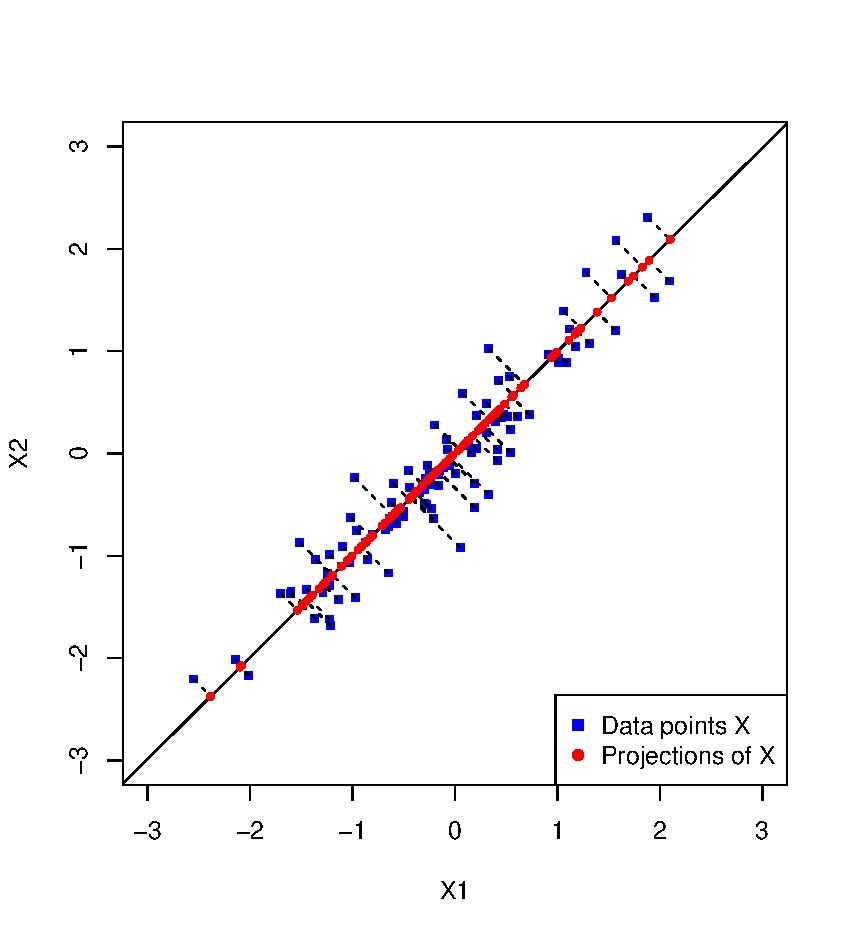
\includegraphics[scale=0.8]{pcapcapca.pdf}
        \caption{The blue squares present the data points $\boldsymbol{x}_1,\boldsymbol{x}_2,\ldots,\boldsymbol{x}_n$, and the red dots present their projections $\boldsymbol{P}\boldsymbol{x}_1, \boldsymbol{P}\boldsymbol{x}_2,\ldots, \boldsymbol{P}\boldsymbol{x}_n$ on $V^*$ (see Eq.~\eqref{eq: V star in HW question}).}
        \label{fig: pcapcapca}
    \end{figure}
\end{enumerate}
\pagebreak

    \color{blue}
        Here is the final plot: 

        \begin{center}
            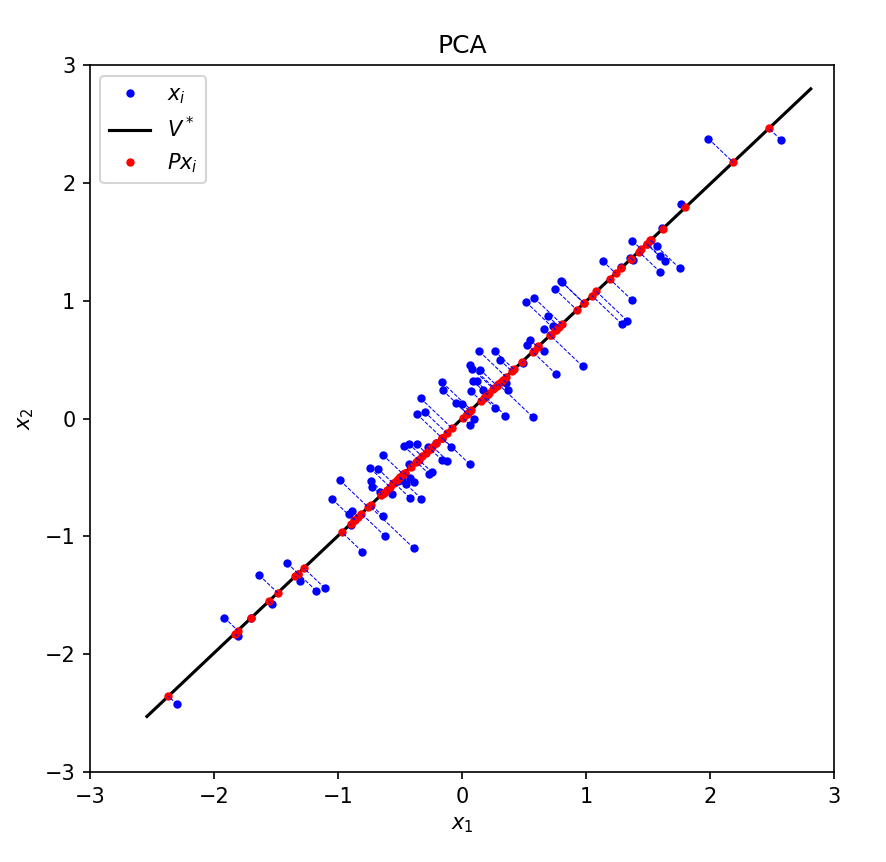
\includegraphics[width=\textwidth]{PCA.png}
        \end{center}

        Here are the numerical results 

        \begin{center}
            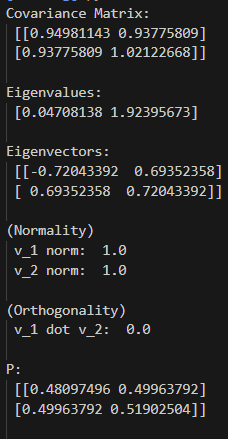
\includegraphics[width=0.6\textwidth]{Numeric results.png}
        \end{center}

        And here is the code I used to generate it. Note that I needed to generate the epsilon vector using the multivariate normal distribution to get a graph similar to the provided one. Generating 200 iid normal random variables and then reshaping them into a 100-by-2 matrix did work when $\varepsilon_i \sim N(0, 0.4)$ so I hypothesize the problem is simply one of scaling to be visible on the graph. 

        \begin{center}
            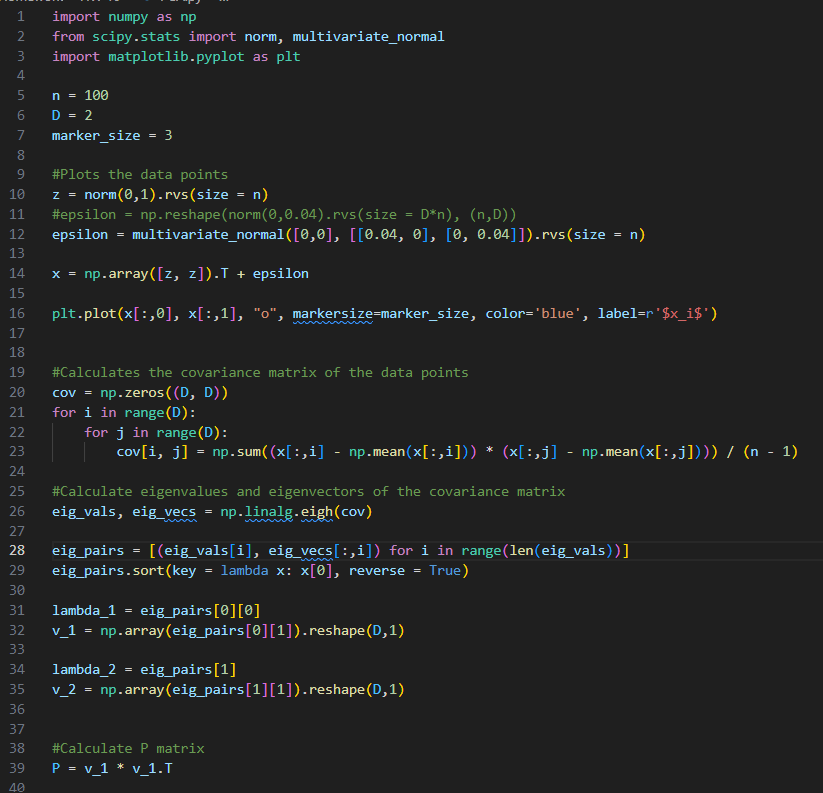
\includegraphics[width=\textwidth]{Code 1.png}
        \end{center}

        \begin{center}
            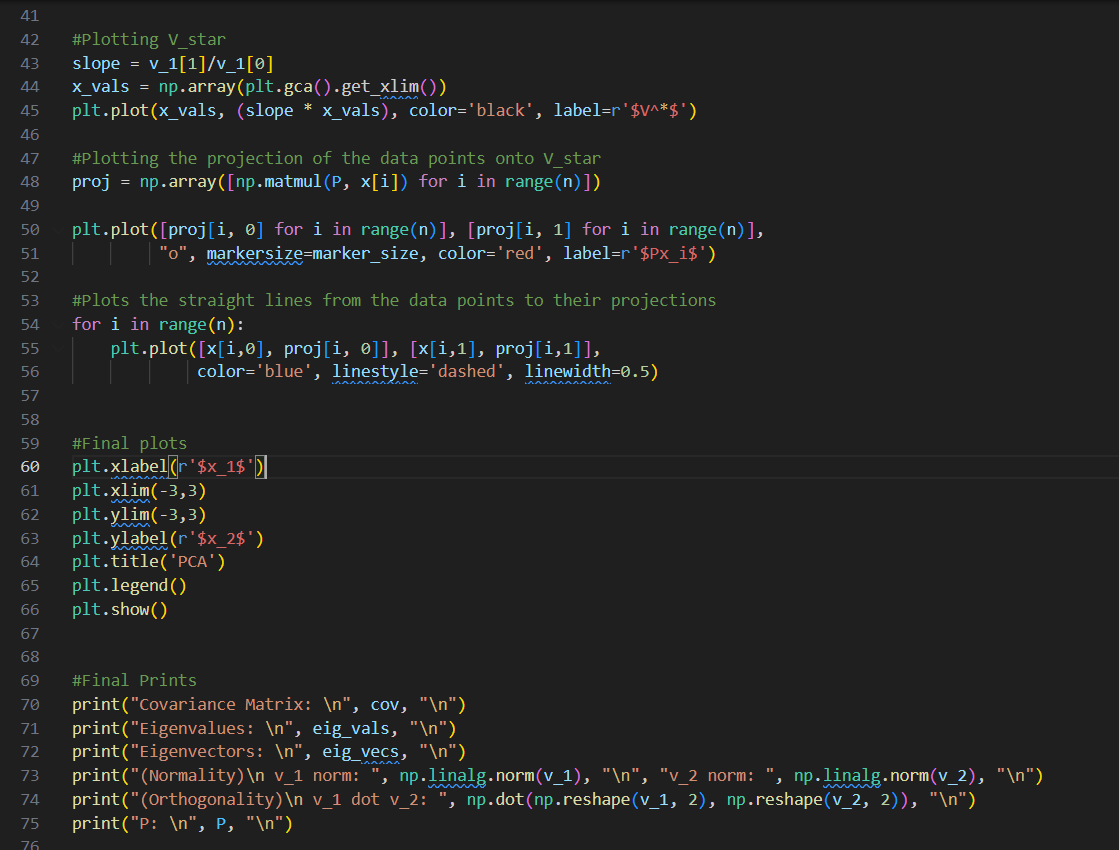
\includegraphics[width=\textwidth]{Code 2.png}
        \end{center}
    \color{black}

\newpage

%\bibliographystyle{plain}
\bibliography{sample}

\end{document}
